%!TEX root = ../template.tex
%%%%%%%%%%%%%%%%%%%%%%%%%%%%%%%%%%%%%%%%%%%%%%%%%%%%%%%%%%%%%%%%%%%%
%% chapter2.tex
%% NOVA thesis document file
%%
%% Chapter with the template manual
%%%%%%%%%%%%%%%%%%%%%%%%%%%%%%%%%%%%%%%%%%%%%%%%%%%%%%%%%%%%%%%%%%%%

\typeout{NT FILE chapter2.tex}%

\chapter{Quadro Teorico: Complessità ed efficienza}\label{chapt:2}
% \glsresetall



\section{Complessità Computazionale}

La complessità computazionale si riferisce allo studio dei requisiti di risorse degli algoritmi, concentrandosi principalmente sulle risorse di tempo e spazio in funzione della dimensione dell'input. Questo campo categorizza i problemi in base alle risorse minime necessarie per risolverli, fornendo un quadro teorico per comprendere la difficoltà intrinseca dei problemi computazionali e l'efficienza degli algoritmi progettati per risolverli. ~\cite{GareyJohnson1979}

\subsection{Complessità Temporale}

La complessità temporale è una misura della quantità di tempo di calcolo che un algoritmo impiega per completarsi in funzione della lunghezza dell'input. Viene spesso espressa utilizzando la notazione Big O, che descrive il limite superiore del tasso di crescita del tempo di esecuzione ~\cite{BigONotation}. Comprendere la complessità temporale di un algoritmo è cruciale per prevederne la scalabilità e la fattibilità nelle applicazioni pratiche, soprattutto per i problemi noti per essere computazionalmente intensivi, come il Problema del Viaggiatore (TSP).

Il \gls{TSP}, essendo \gls{NP} -hard, non ha una soluzione in tempo polinomiale nota che possa risolvere in modo efficiente tutte le istanze del problema. L'approccio a forza bruta per il \gls{TSP}, ad esempio, ha una complessità temporale fattoriale (\(O(n!)\)), rendendolo computazionalmente irrealizzabile anche per istanze del problema di dimensioni moderatamente grandi. Ciò ha portato all'esplorazione di vari algoritmi euristici e meteuristici che mirano a soluzioni accettabili in tempo polinomiale (\(O(n^k)\)), dove \(k\) è una costante, scambiando precisione per efficienza e applicabilità pratica.~\cite{Dorigo1996}


\begin{figure}[h]
	\centering
	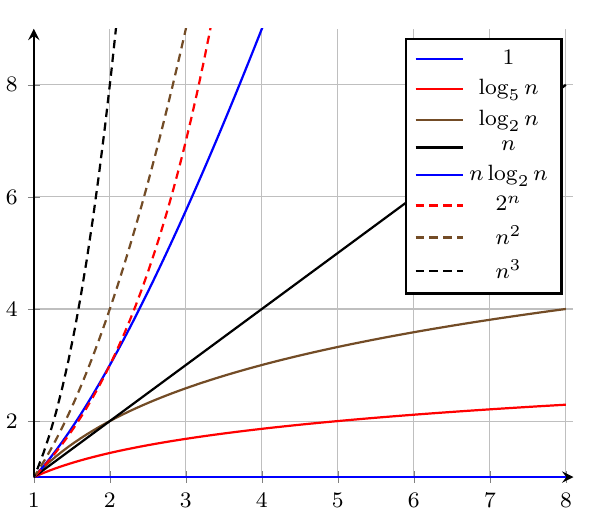
\begin{tikzpicture}
		\begin{axis}
			[
				axis lines = left,
				xmin=1, xmax=8.1, ymin=1, ymax=9,
				domain=0:8, samples=100, no markers, thick, grid=both,
				xlabel = \(n\), ylabel = {\(f(n)\)},
				label style = {overlay},       % Has he same effect as
				ticklabel style = {overlay},   % trim axis [left|right]
				legend entries = {
						$1$,
						$\log_{5}n$,
						$\log_{2}n$,
						$n$,
						$n\log_{2}n$,
						$2^{n}$,
						$n^{2}$,
						$n^{3}$,
					},
				every axis/.style = {font=\footnotesize},
				label style = {font=\normalsize},
			]
			\addplot+ {1};
			\addplot+ {1 + ln(x)/ln(5)};
			\addplot+ {1 + ln(x)/ln(2)};
			\addplot+ {x};
			\addplot+ {1 + x*ln(x)/ln(2)};
			\addplot+ {2^x-1};
			\addplot+ {x^2};
			\addplot+ {x^3};
		\end{axis}
	\end{tikzpicture}
	\vspace{1.0cm}
	\caption{Tasso di crescita delle diverse complessità}
\end{figure}


\begin{table}[h]
	\centering
	\caption{Numero di possibili permutazioni per numero di città}
	\begin{tabular}{c l}
		\toprule
		Numero città & Numero Permutazioni                \\
		\midrule
		4            & 24                                 \\
		5            & 120                                \\
		6            & 720                                \\
		7            & 5,040                              \\
		8            & 40,320                             \\
		9            & 362,880                            \\
		10           & 3,628,800                          \\
		11           & 39,916,800                         \\
		12           & 479,001,600                        \\
		13           & 6,227,020,800                      \\
		14           & 87,178,291,200                     \\
		15           & 1,307,674,368,000                  \\
		16           & 20,922,789,888,000                 \\
		17           & 355,687,428,096,000                \\
		18           & 6,402,373,705,728,000              \\
		19           & 121,645,100,408,832,000            \\
		20           & 2,432,902,008,176,640,000          \\
		25           & 15,511,210,043,330,985,984,000,000 \\
		\bottomrule
	\end{tabular}
\end{table}

\subsection{Complessità Spaziale}

La complessità spaziale misura la quantità totale di memoria di cui un algoritmo ha bisogno per eseguirsi fino al completamento in funzione della dimensione dell'input. Come la complessità temporale, la complessità di spazio è cruciale per valutare l'efficienza di un algoritmo, in particolare in scenari in cui le risorse di memoria sono limitate. Nel contesto del \gls{TSP} e di problemi di ottimizzazione simili, la complessità spaziale di un algoritmo può influire significativamente sulla sua usabilità in applicazioni del mondo reale, dove le soluzioni spesso devono essere calcolate in tempo reale o su hardware con capacità di memoria limitate.~\cite{HeldKarp1962}.

Ad esempio, gli approcci di programmazione dinamica per il \gls{TSP}, come l'algoritmo di Held-Karp, offrono una complessità temporale più favorevole rispetto alla forza bruta (\(O(n^2 2^n)\)) ma a costo di una complessità di spazio esponenziale (\(O(n^2)\)). Tali compromessi tra complessità temporale e spaziale sono considerazioni centrali nella progettazione degli algoritmi, soprattutto quando si sviluppano nuovi algoritmi destinati a istanze di problemi su larga scala, come quelle riscontrate in applicazioni di logistica e routing.

\section{Il Problema \gls{P} vs. \gls{NP} }

Il problema \gls{P} vs. \gls{NP} è una delle domande irrisolte più fondamentali nell'informatica. Chiede se ogni problema la cui soluzione può essere rapidamente verificata (in tempo polinomiale) da un computer può anche essere rapidamente risolto (in tempo polinomiale) da un computer. La classe \gls{P} consiste di problemi che possono essere risolti rapidamente, mentre la classe \gls{NP} consiste di problemi per i quali una soluzione proposta può essere rapidamente verificata.~\cite{PvsNP}.

\begin{figure}[h]
	\centering
	% TODO: Use venndiagram package to draw the diagram
	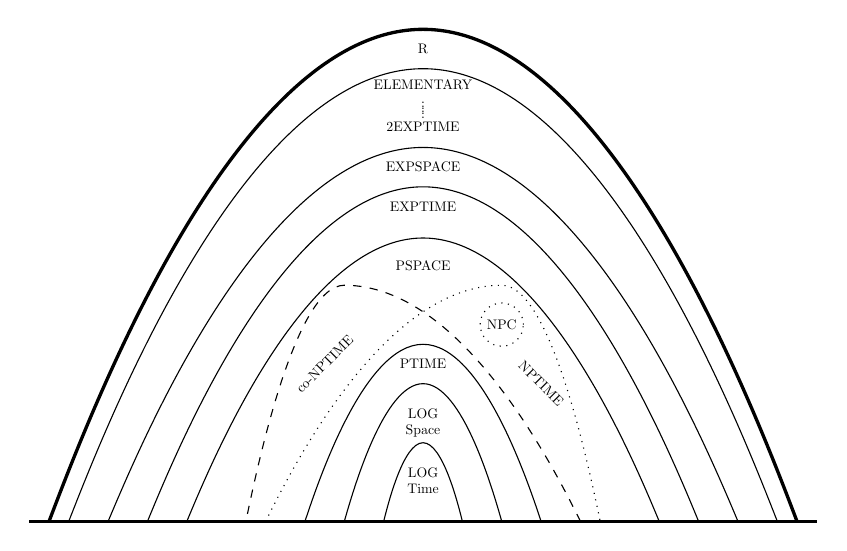
\begin{tikzpicture}[scale=0.5, every node/.append style={scale=0.5}]
		\pgftransformscale{1}

		%%% HELP LINES - uncomment to design/extend
		% \draw[step=1cm,gray,very thin] (-10,0) grid (10,12);
		% \node at (0,0) {\textbf{(0,0)}};

		%% Horizontal bar
		\draw[very thick] (10,0) -- (-10,0);

		% LOG TIME
		\draw (-1,0) parabola bend (0,2) (1,0) ;
		\node at (0,1) {
			\begin{tabular}{c}
				LOG \\ Time
			\end{tabular}
		};

		% LOG SPACE
		\draw (-2,0) parabola bend (0,3.5) (2,0);
		\node at (0,2.5) {
			\begin{tabular}{c}
				LOG \\ Space
			\end{tabular}
		};

		% PTIME
		\draw (-3,0) parabola bend (0,4.5) (3,0);
		\node at (0,4) {PTIME};

		% NP
		\draw[dotted] (-4,0) parabola bend (2,6) (4.5,0);
		\node[rotate=-45] at (3,3.5) {NPTIME};

		% NP-complete
		\node[circle,dotted,draw] at (2,5) {NPC};

		% Co-NP
		\draw[dashed] (4,0) parabola bend (-2,6) (-4.5,0);
		\node[rotate=45] at (-2.5,4) {co-NPTIME};

		% PSPACE
		\draw (-6,0) parabola bend (0,7.2) (6,0);
		\node at (0,6.5) {PSPACE};

		% EXPTIME
		\draw (-7,0) parabola bend (0,8.5) (7,0);
		\node at (0,8) {EXPTIME};

		% EXPTIME
		\draw (-8,0) parabola bend (0,9.5) (8,0);
		\node at (0,9) {EXPSPACE};

		% ELEMENTARY
		\draw (-9,0) parabola bend (0,11.5) (9,0);
		\node at (0,10.5) {$\vdots$};
		\node[anchor=north] at (0,11.4) {
			\begin{tabular}{c}
				ELEMENTARY \\
				$\vdots$   \\
				2EXPTIME
			\end{tabular}
		};

		% RECURSIVE
		\draw[very thick] (-9.5,0) parabola bend (0,12.5) (9.5,0);
		\node at (0,12) {R};
	\end{tikzpicture}
	\caption{Classificazione dei problemi computazionali}
\end{figure}
\subsection{Definizione e Rilevanza}

Formalmente, un problema appartiene alla classe \gls{P} se può essere risolto in tempo polinomiale, il che significa che la quantità di tempo necessaria per risolvere il problema cresce in modo polinomiale con la dimensione dell'input. La classe \gls{NP} , d'altra parte, comprende i problemi per i quali una soluzione data può essere verificata in tempo polinomiale. Il problema \gls{P} vs. \gls{NP} chiede essenzialmente se queste due classi sono uguali; cioè, se ogni problema che può essere verificato rapidamente può anche essere risolto rapidamente.

La rilevanza del problema \gls{P} vs. \gls{NP} risiede nelle sue implicazioni per un vasto campo di discipline, dalla crittografia e la progettazione di algoritmi ai processi decisionali e oltre. Una prova che \gls{P} è uguale a \gls{NP} potrebbe potenzialmente rivoluzionare i campi della matematica e dell'informatica, consentendo soluzioni efficienti a una moltitudine di problemi complessi attualmente considerati intrattabili. Al contrario, provare che \gls{P} non è uguale a \gls{NP} formalizzerebbe la difficoltà computazionale intrinseca di questi problemi.

\subsection{Implicazioni per il \gls{TSP}}

La classificazione del \gls{TSP} come \gls{NP} -hard sottolinea la complessità e le sfide computazionali associate al trovare una soluzione esatta per grandi istanze del problema. Questa classificazione ha implicazioni significative sia per la ricerca teorica che per le applicazioni pratiche nel campo. Implica che a meno che \gls{P} non sia uguale a \gls{NP} - una questione che rimane uno dei problemi irrisolti più fondamentali nell'informatica - non ci si dovrebbe aspettare di scoprire un algoritmo in grado di risolvere rapidamente (in tempo polinomiale) e accuratamente ogni istanza del \gls{TSP}. Questa consapevolezza ha spostato il focus di gran parte della ricerca sul \gls{TSP} verso lo sviluppo di algoritmi euristici e meteuristici, che mirano a trovare soluzioni sufficientemente buone in un lasso di tempo ragionevole, piuttosto che inseguire l'elusivo obiettivo di una soluzione esatta per tutte le possibili istanze.~\cite{Karp1972}.

Inoltre, le implicazioni del fatto che il \gls{TSP} sia \gls{NP} -hard si estendono oltre lo sviluppo degli algoritmi. Influenza il modo in cui i problemi vengono modellati in scenari pratici in cui sorgono problemi simili al \gls{TSP}, come la logistica e il routing, la progettazione di reti e la pianificazione. In queste applicazioni, l'enfasi è spesso rivolta al trovare soluzioni che si avvicinino all'ottimale ma possano essere ottenute molto più rapidamente di quanto permetterebbe un algoritmo esatto. Questo approccio consente all'industria di raggiungere efficienza e risparmi di costi anche quando si affrontano problemi di routing e pianificazione complessi.

Inoltre, lo studio del \gls{TSP} e del suo posto nella classe \gls{NP}-hard ha stimolato l'interesse nell'esplorare i limiti del potere computazionale e comprendere la difficoltà intrinseca dei vari problemi computazionali. Sfida i ricercatori a innovare costantemente e a trovare nuovi modi di affrontare la risoluzione dei problemi in matematica computazionale e informatica. Pertanto, le implicazioni della classificazione del \gls{TSP} risuonano sia nello studio accademico della teoria degli algoritmi che nelle considerazioni pratiche sull'applicazione di queste teorie in situazioni del mondo reale.

\section{Complessità del \gls{TSP}}

La dimostrazione che il \gls{TSP} è \gls{NP} -hard è stata presentata per la prima volta da Richard M. Karp nel 1972. Il lavoro di Karp, parte di un articolo seminale che identificava 21 problemi \gls{NP} -completi, ha gettato le basi per comprendere i limiti computazionali delle soluzioni algoritmiche per il \gls{TSP} e problemi simili. Dimostrando che la versione decisionale del \gls{TSP} (determinare se esiste un tour di una data lunghezza o inferiore) è \gls{NP}-complete, Karp ha dimostrato in modo efficace che la versione di ottimizzazione del \gls{TSP}, in cui l'obiettivo è trovare il tour più breve possibile, è \gls{NP} -hard.

La dimostrazione di Karp impiega una tecnica nota come riduzione, in cui un problema \gls{NP} -completo noto viene trasformato in un'istanza del \gls{TSP} in tempo polinomiale. Questo metodo illustra che se un algoritmo in tempo polinomiale potesse risolvere il \gls{TSP}, potrebbe, per estensione, risolvere tutti i problemi in \gls{NP} , una proposizione che rimane non verificata. Pertanto, la dimostrazione non solo identifica il \gls{TSP} come un problema fondamentalmente impegnativo, ma approfondisce anche la nostra comprensione del panorama della complessità computazionale.

Le implicazioni dell'\gls{NP}-hardness del \gls{TSP} sono di vasta portata nel campo della progettazione di algoritmi. Indica che, a meno che P=NP, non esiste un algoritmo in grado di risolvere efficientemente tutte le istanze del \gls{TSP}. Questa consapevolezza ha stimolato lo sviluppo di vari algoritmi euristici e di approssimazione, che mirano a soluzioni praticamente buone, anche se non sempre ottimali, entro limiti di tempo computazionale ragionevoli.

\begin{table}[h]
	\centering
	\resizebox{\textwidth}{!}{
		\begin{tabular}{@{}lcccc@{}}
			\toprule
			\textbf{Algoritmo} & \textbf{Complessità Temporale} & \textbf{Complessità Spaziale} & \textbf{Descrizione}                                     & \textbf{Vantaggi}                        & \textbf{Svantaggi}                     \\ \midrule
			Held-Karp          & \(O(n^2 2^n)\)                 & \(O(n^2)\)                    & Algoritmo esatto che utilizza la programmazione dinamica & Fornisce soluzione ottimale              & Inattuabile per grandi \(n\)           \\
			Nearest Neighbor   & \(O(n^2)\)                     & \(O(n)\)                      & Algoritmo euristico greedy                               & Semplice e veloce                        & Spesso lontano dall'ottimale           \\
			Christofides       & \(O(n^3)\)                     & \(O(n^2)\)                    & Algoritmo di approssimazione con rapporto di 3/2         & Migliore approssimazione per TSP metrico & Ancora non esatto                      \\
			Algoritmi Genetici & \(O(n^2)\)                     & \(O(n)\)                      & Algoritmo metaeuristico ispirato alla selezione naturale & Flessibile e adattabile                  & Nessuna garanzia di soluzione ottimale \\ \bottomrule
		\end{tabular}
	}
	\caption{Confronto tra Diversi Algoritmi per TSP}
\end{table}

\subsection{Impatto sulla Progettazione degli Algoritmi}

L'\gls{NP}-hardness del \gls{TSP} ha un profondo impatto sulla progettazione degli algoritmi per risolverlo, favorendo lo sviluppo di varie strategie volte a superare gli ostacoli computazionali:

\begin{itemize}
	\item \textbf{Algoritmi Esatti:} Nonostante l'\gls{NP}-hardness del \gls{TSP}, sono stati ideati algoritmi esatti, come l'algoritmo di Held-Karp. Questi algoritmi garantiscono una soluzione ottimale, ma lo fanno a un costo computazionale che aumenta esponenzialmente con le dimensioni del problema, rendendoli impraticabili per istanze di grandi dimensioni.
	\item \textbf{Approcci Euristici:} Per affrontare istanze di \gls{TSP} più grandi, vengono impiegati algoritmi euristici. Questi algoritmi non garantiscono una soluzione ottimale, ma possono spesso trovare buone soluzioni in una frazione del tempo richiesto dai metodi esatti. Esempi includono l'algoritmo del Vicino più Vicino e l'algoritmo di Christofides.
	\item \textbf{Algoritmi Meteuristici:} Per istanze ancora più complesse, gli approcci meteuristici, come gli Algoritmi Genetici e l'Ottimizzazione della Colonia di Formiche, offrono strategie flessibili che esplorano lo spazio delle soluzioni in modo più ampio, mirando a sfuggire agli ottimi locali e avvicinarsi più efficacemente agli ottimi globali. Queste tecniche attingono ispirazione dai processi naturali e hanno il vantaggio dell'adattabilità a diverse istanze di problema.
	\item \textbf{Algoritmi di Approssimazione:} Data l'\gls{NP}-hardness del \gls{TSP}, gli algoritmi di approssimazione che forniscono garanzie dimostrabile sulla vicinanza della soluzione all'ottimo sono particolarmente preziosi. Questi algoritmi sono particolarmente pertinenti per specifiche varianti del \gls{TSP}, come il \gls{TSP} Metrico, dove possono sfruttare la disuguaglianza triangolare per limitare la qualità della soluzione.
\end{itemize}

L'\gls{NP}-hardness del \gls{TSP} sottolinea quindi non solo la difficoltà intrinseca del problema, ma catalizza anche l'innovazione nella progettazione degli algoritmi, spingendo i confini di ciò che può essere raggiunto computazionalmente entro i vincoli della complessità computazionale.
